\section{Convolutional Neural Network (CNN)}
    Convolutional neural networks (CNN) are a regularized type of feed-forward neural network that learns feature engineering by itself via filters (or kernel) optimization. \cite{convnet}
    \par\vspace{1em}
    
    \begin{figure}[h]
            \centering
            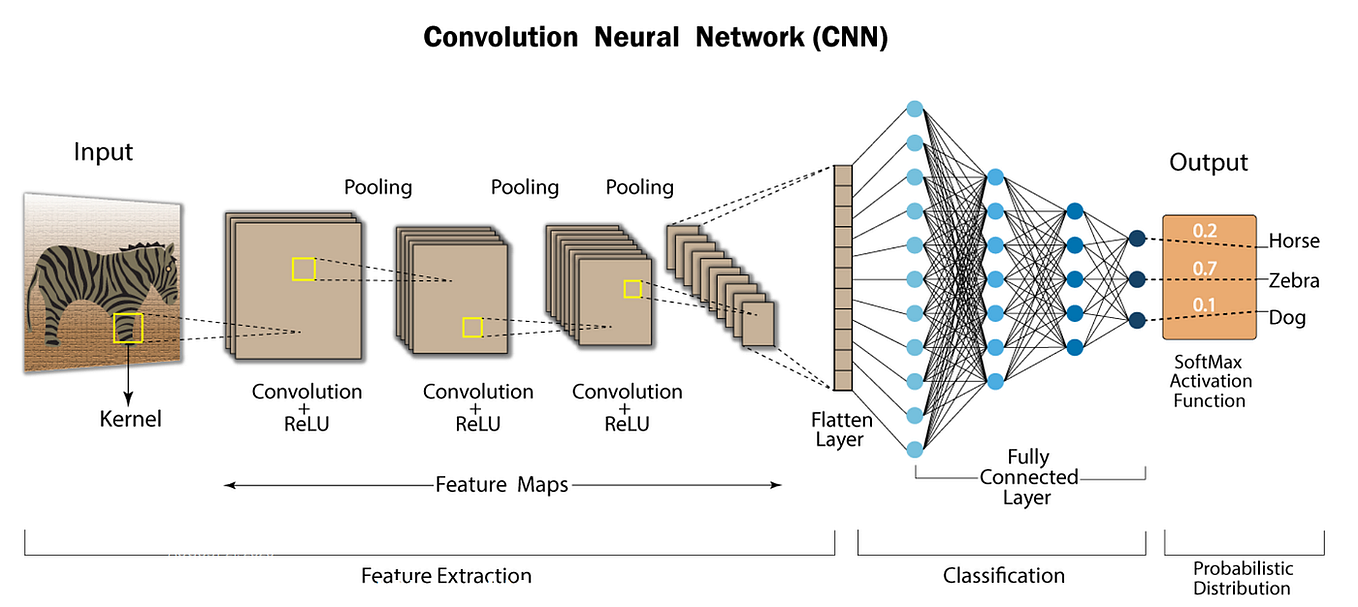
\includegraphics[width=1\textwidth]{graphics/chapter3/general cnn classification model.png}
            \caption{A typical ConvNet Classification Model, Source: \cite{convnet-fig}} 
            \label{fig:cnn1}
        \end{figure}
        
        
    \subsection{Architecture of CNN}
    A convolutional neural network consists of an input layer, hidden layers and an output layer. In a convolutional neural network, the hidden layers include one or more layers that perform convolutions. Typically this includes a layer that performs a dot product of the convolution kernel with the layer's input matrix. This product is usually the Frobenius inner product, and its activation function is commonly ReLU. As the convolution kernel slides along the input matrix for the layer, the convolution operation generates a feature map, which in turn contributes to the input of the next layer. This is followed by other layers such as pooling layers, fully connected layers, and normalization layers. Here it should be noted how close a convolutional neural network is to a matched filter\cite{convnet-1}.
        \subsubsection{Convolution Layers}
        In a CNN, the input is a tensor with shape:        
        \[(\text{number of inputs}) * (\text{input height}) * (\text{input width}) * (\text{input channels})\]
        After passing through a convolutional layer, the image becomes abstracted to a feature map, also called an activation map, with shape:
        \[(\text{number of inputs}) * (\text{feature map height}) * (\text{feature map width}) * (\text{feature map channels})\]
        \par \vspace{1em}
        Convolutional layers convolve the input and pass its result to the next layer. This is similar to the response of a neuron in the visual cortex to a specific stimulus\cite{convnet-2}. Each convolutional neuron processes data only for its receptive field.
        
        \subsubsection{Pooling Layers}
        Convolutional networks may include local and/or global pooling layers along with traditional convolutional layers. Pooling layers reduce the dimensions of data by combining the outputs of neuron clusters at one layer into a single neuron in the next layer. Local pooling combines small clusters, tiling sizes such as 2 × 2 are commonly used. Global pooling acts on all the neurons of the feature map.There are two common types of pooling in popular use: max and average. Max pooling uses the maximum value of each local cluster of neurons in the feature map, while average pooling takes the average value \cite{convnet-3}.
        
        \subsubsection{Fully Connected Layers}
        Fully connected layers connect every neuron in one layer to every neuron in another layer. It is the same as a traditional multilayer perceptron neural network (MLP). The flattened matrix goes through a fully connected layer to classify the image
        
        \subsubsection{Activation Function}
        Activation function decides whether a neuron should be activated or not by calculating the weighted sum and further adding bias to it. The purpose of the activation function is to introduce non-linearity into the output of a neuron. 
        
        \subsubsection{Rectified Linear Unit Activation Function (RELU)}
        ReLU applies the non-saturating activation function\par
        \begin{center}
            \(f(z) = max(0, z)\)    
        \end{center}

        \begin{figure}
            \centering
            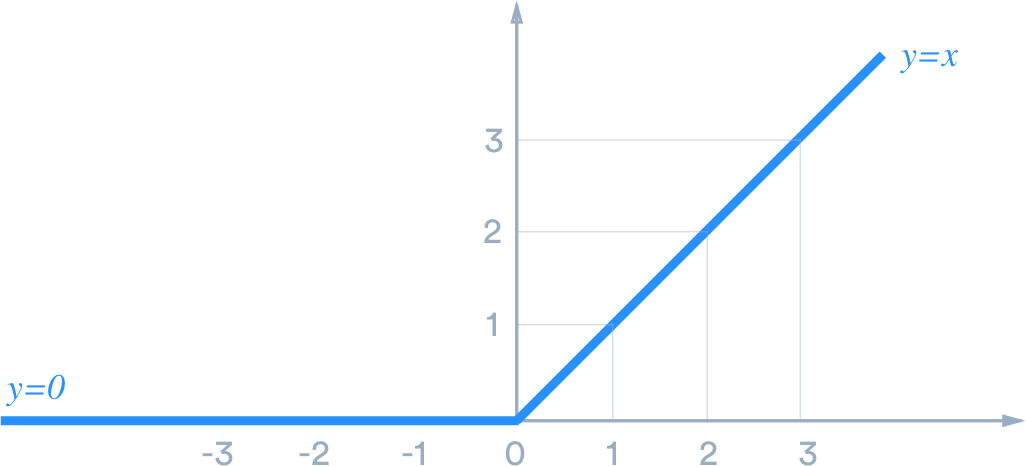
\includegraphics[width=0.5\linewidth]{graphics//chapter3/relu.png}
            \caption{Rectified Linear Unit Activation Function (ReLU) }
            \label{fig:relu}
        \end{figure}
        
        It effectively removes negative values from an activation map by setting them to zero.
        Rectified Linear Unit (ReLU) or rectifier activation function introduces the property of nonlinearity to a deep learning model and solves the vanishing gradients issue. It interprets the positive part of its argument\cite{relu-0}.\par \vspace{1em}
        
    \subsection{Backpropagation in CNN}
    Backpropagation is a process involved in training a neural network. It takes the error rate of a forward propagation and feeds this loss backward through the neural network layers to adjust the weights. It is the practice of fine-tuning the weights of a neural net based on the error rate (i.e. loss) obtained in the previous epoch (i.e. iteration.) Proper tuning of the weights ensures lower error rates, making the model reliable by increasing its generalization.
